\section{Training on more complex data patterns}
\label{sec:more_patterns}

The observations presented in the previous sections can be used to select an 'overall better' model.

\begin{table}[h]
\begin{tabular}{ccccc}
\hline\hline layer    & type    & outputs & parameters & activation\\ \hline
input    & Dense   & 2       & 6     & softplus \\
dense\_1 & Dense   & 20      & 60    & softplus \\
dense\_2 & Dense   & 20      & 420   & softplus \\
output   & Dense   & 1       & 21    & sigmoid  \\ \hline\hline
\multicolumn{3}{c}{dropout}  & \multicolumn{2}{c}{no} \\
\multicolumn{3}{c}{initialization}  & \multicolumn{2}{c}{glorot normal} \\
\multicolumn{3}{c}{optimizer}  & \multicolumn{2}{c}{Nadam} \\ \hline\hline
\end{tabular}
\caption{\label{tab:best_model}Layout of the best DNN we have tweaked using the results of section \ref{sec:gridsearches} and \ref{sec:data_init}.}
\end{table}

Finally, we have tested the application of such model to learn more complex patterns in 2D data. We have selected a set of more complex labeling functions in order to find some edge cases. The full list of functions is shown in the attached Jupyter notebook, whereas the Figure \ref{fig:predictions_complex} shows some of the most interesting results.

\begin{figure}[b] %htp
  \centering
  \begin{subfigure}{\columnwidth}
  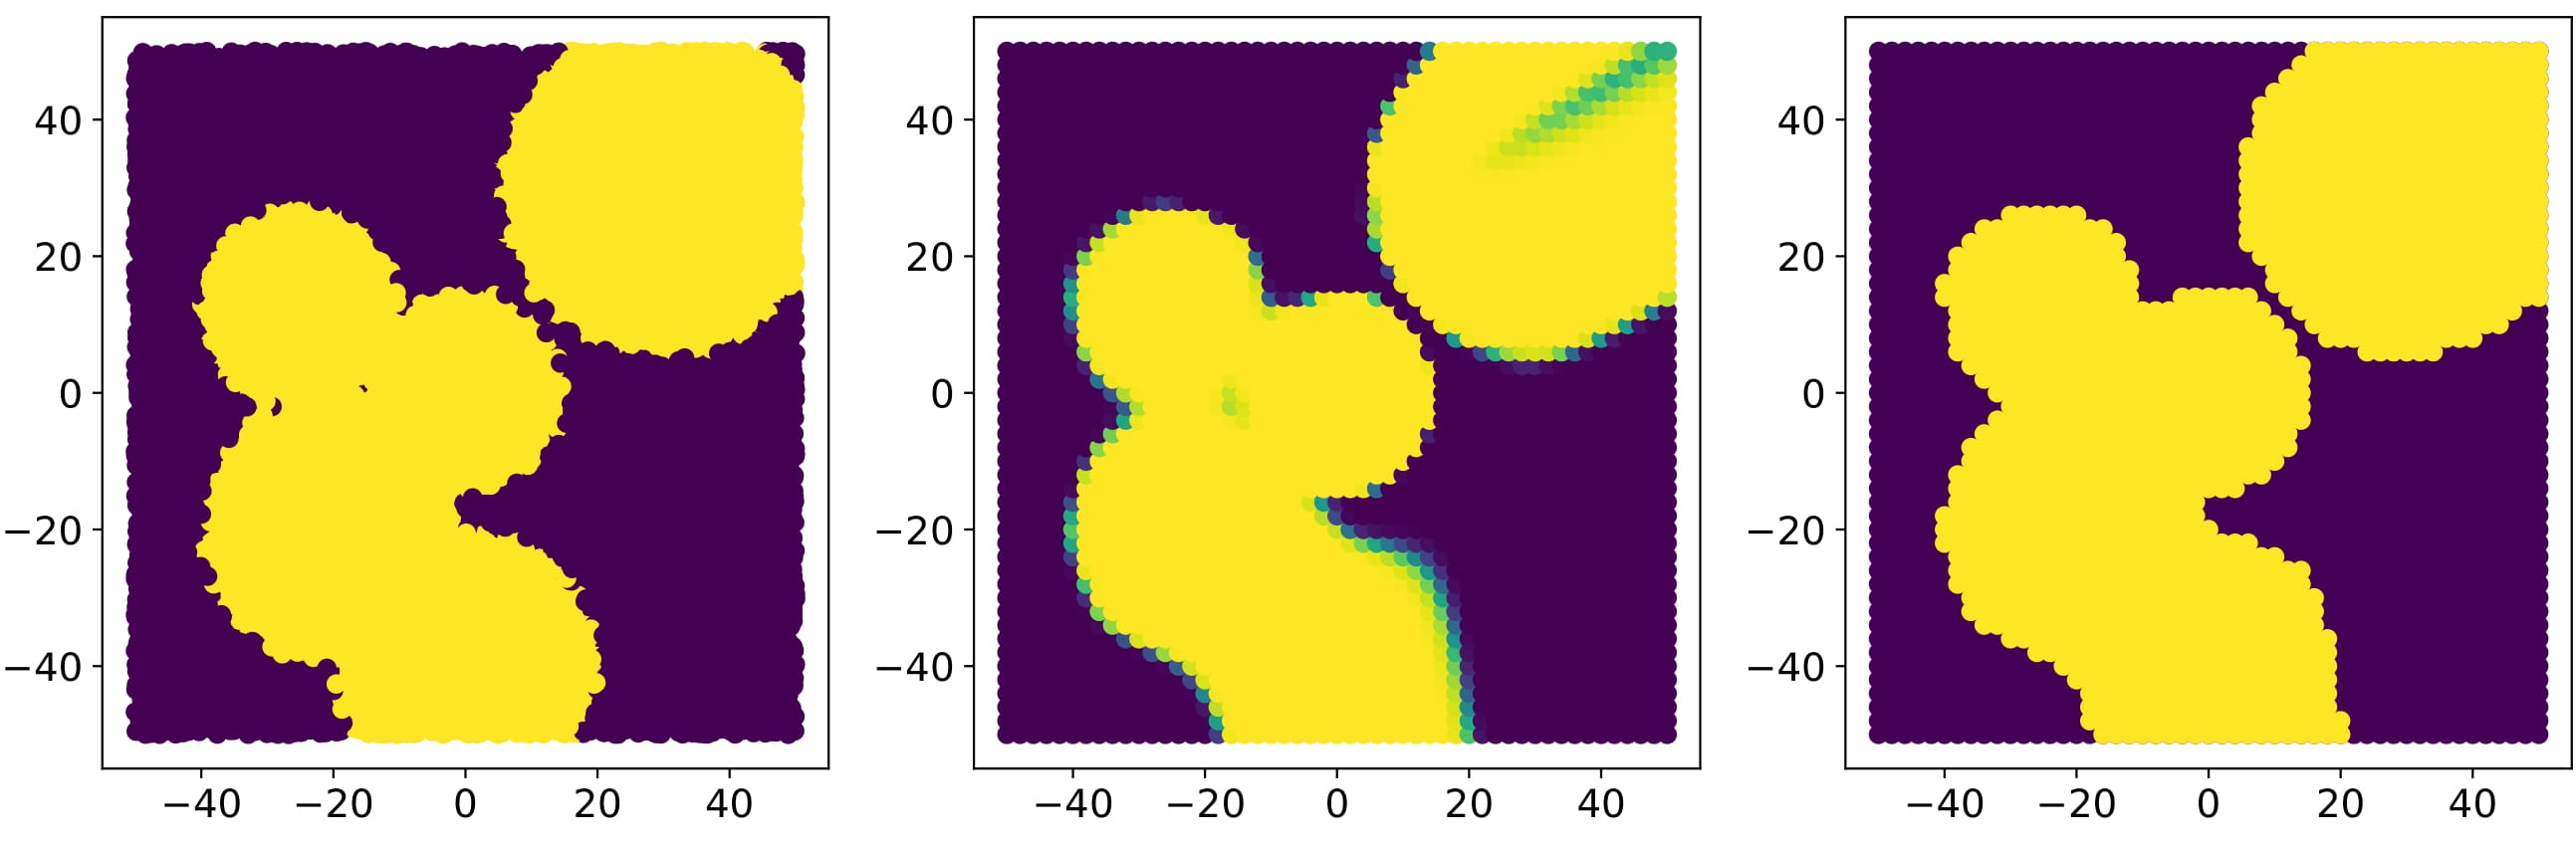
\includegraphics[width=\columnwidth]{multi_sphere_prediction_crop.jpg}
  \caption{\label{fig:predictions_spheres} Multi-sphere.}
  \end{subfigure}
  
  \begin{subfigure}{\columnwidth}
  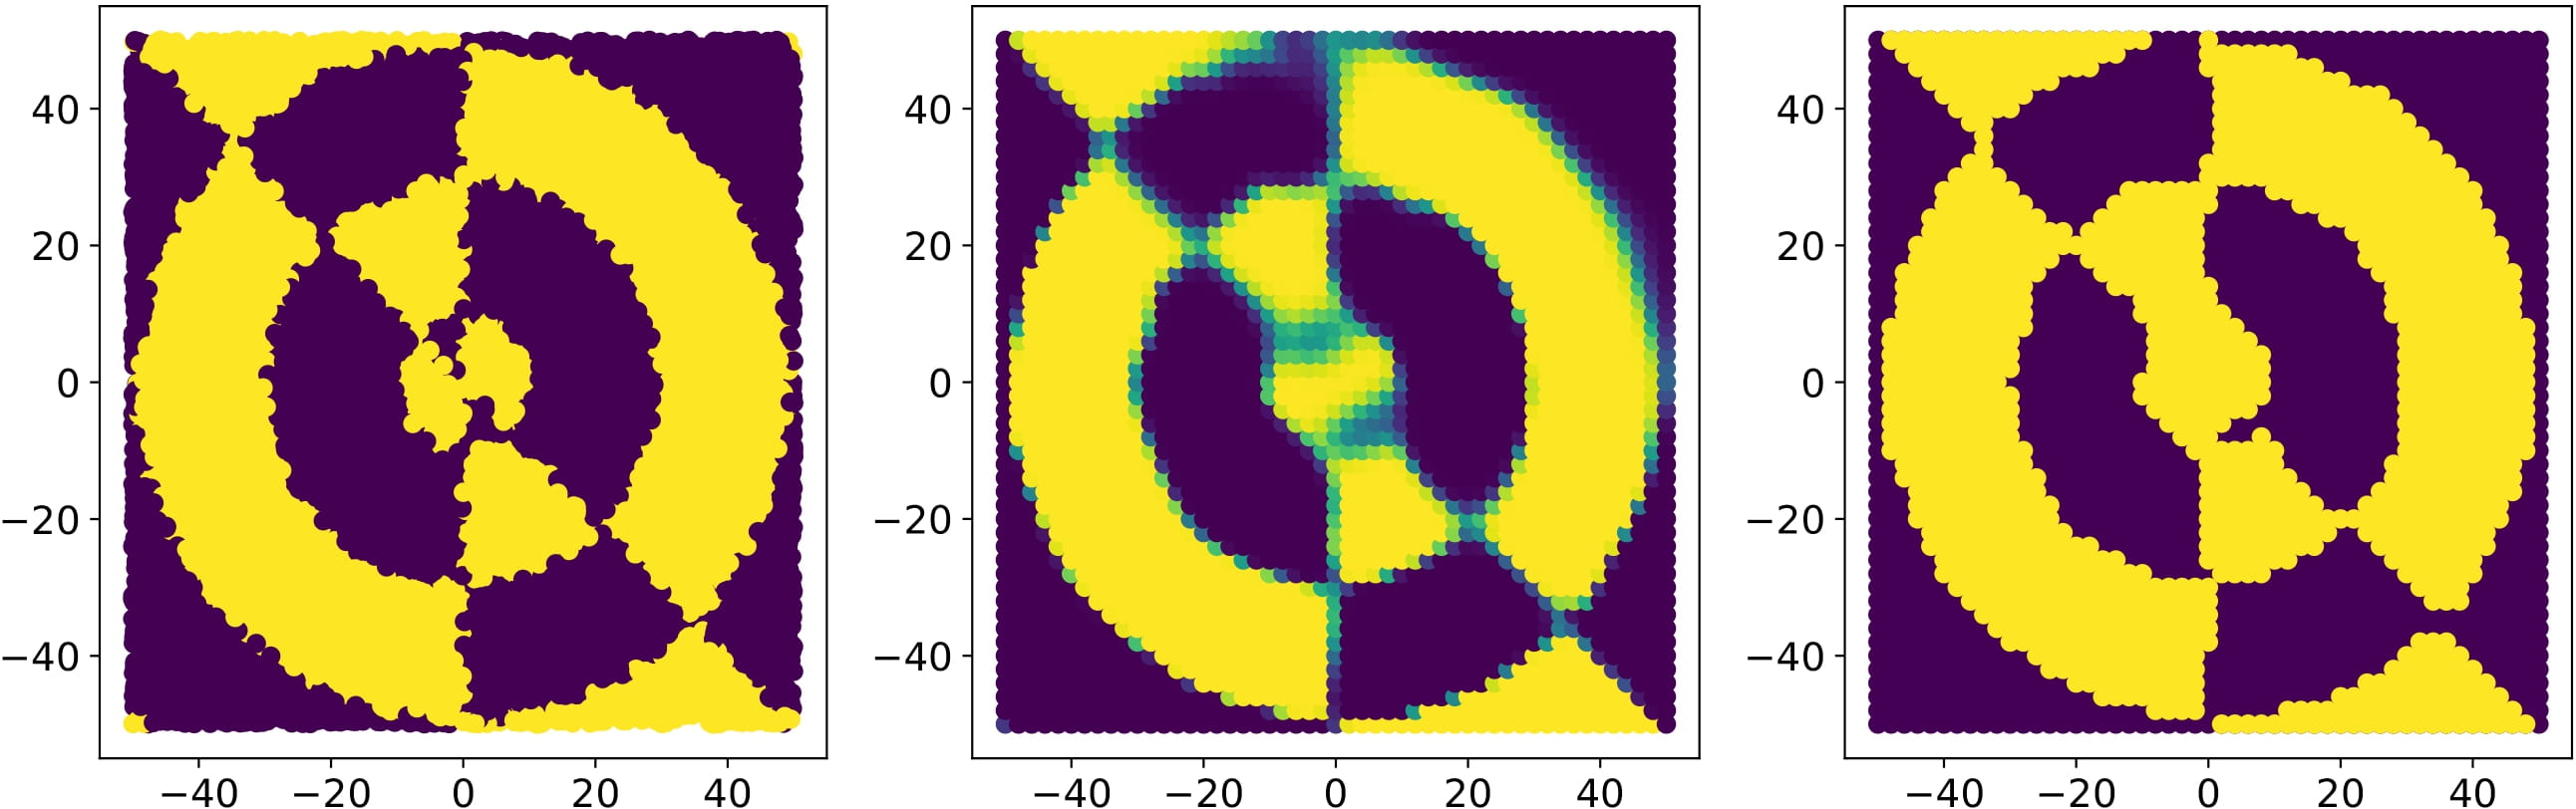
\includegraphics[width=\columnwidth]{baiesi_second_prediction_crop.jpg}
  \caption{\label{fig:predictions_baiesi} Alternative function suggested by Prof. Baiesi.}
  \end{subfigure}
  
  \begin{subfigure}{\columnwidth}
  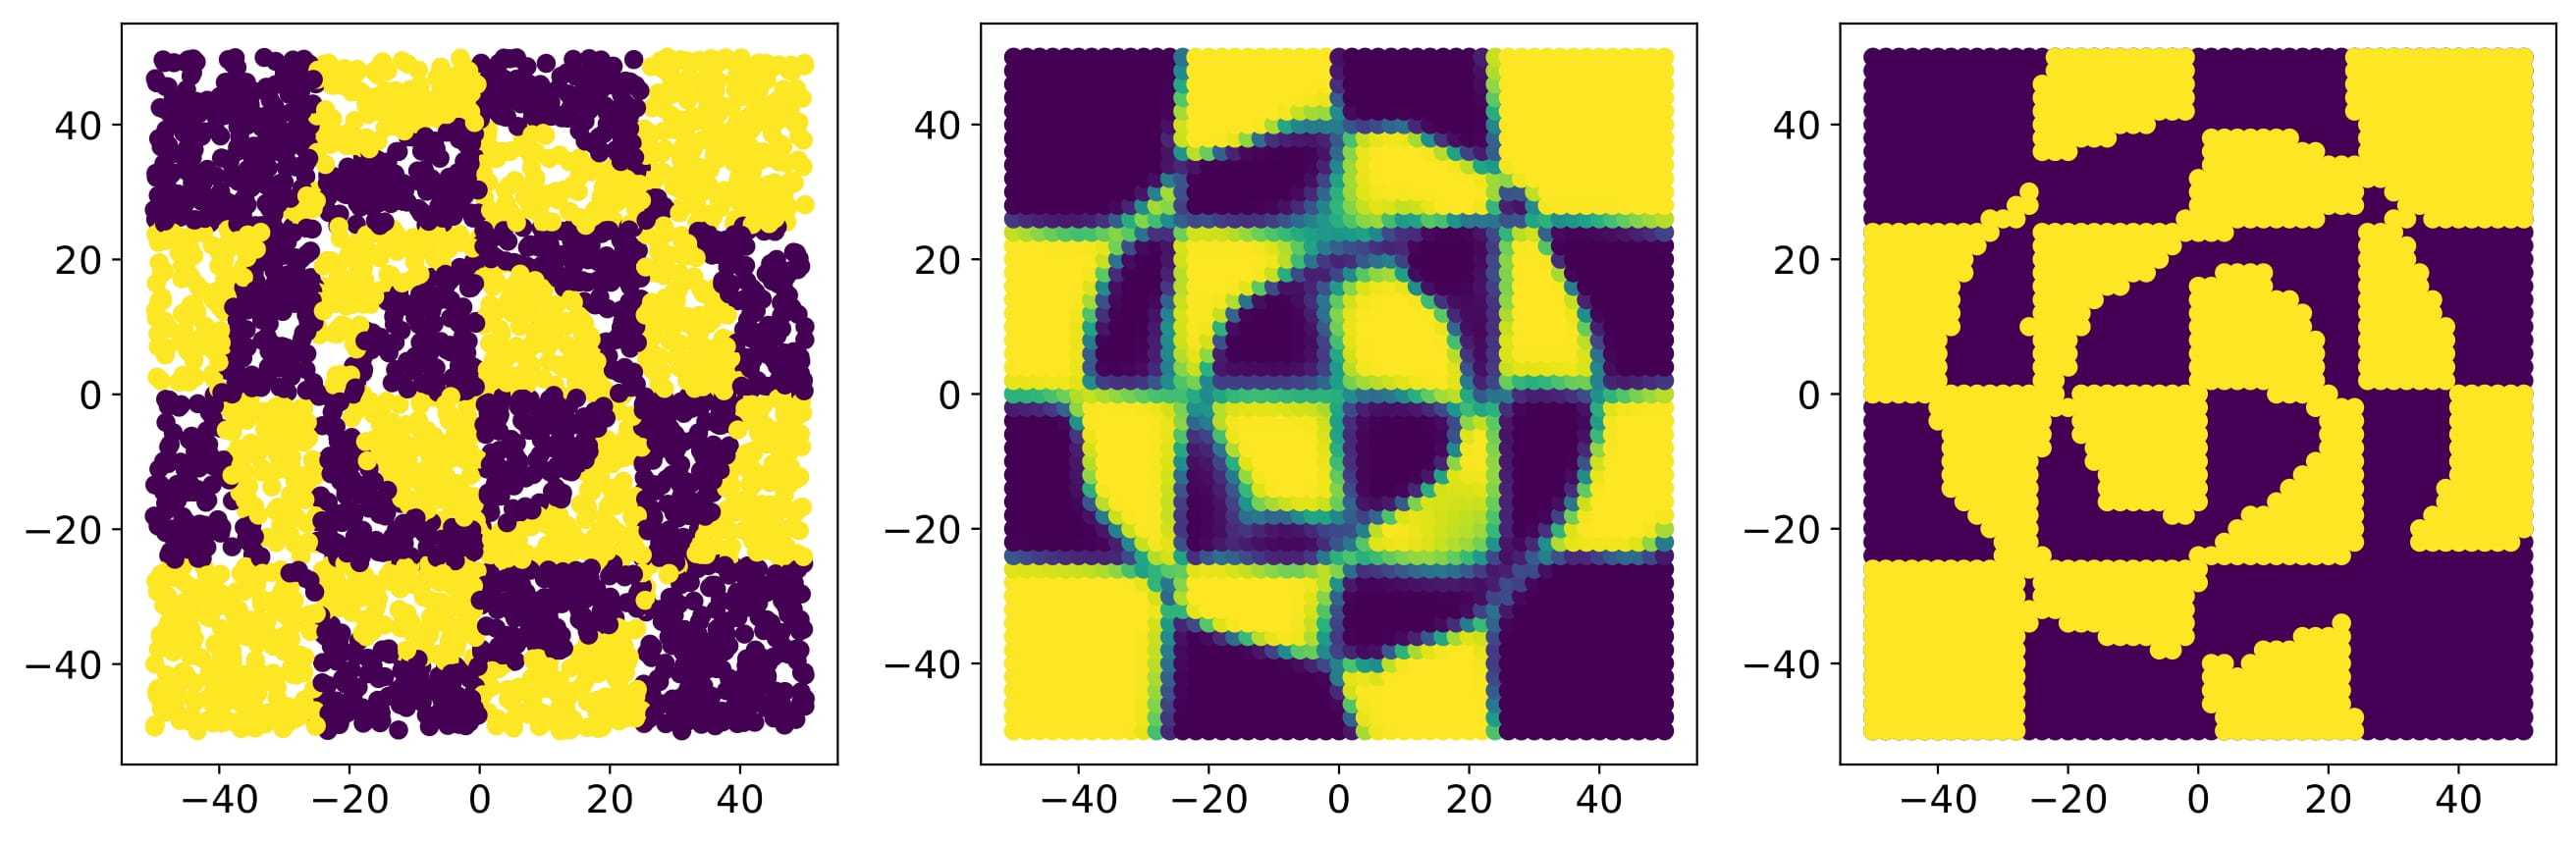
\includegraphics[width=\columnwidth]{mixed_chessboard_prediction_augm_500_crop.jpg}
  \caption{\label{fig:predictions_chessboard} Mixed chessboard. In particular, this model has been trained using the data augmentation technique presented in section \ref{ssec:augmented_dataset}.}
  \end{subfigure}
  
  \caption{\label{fig:predictions_complex}Prediction grids of the best DNN configuration (\ref{tab:best_model}) (2-layers) trained for $> 800$ epochs on various data patterns (of size $20k$). The first figures on the left show the original dataset, while the two other figures show the prediction grids of the DNN model. DNNs with 3 hidden layers are able to achieve the same results but in much less epochs.}
\end{figure}